\documentclass[1p]{elsarticle_modified}
%\bibliographystyle{elsarticle-num}

%\usepackage[colorlinks]{hyperref}
%\usepackage{abbrmath_seonhwa} %\Abb, \Ascr, \Acal ,\Abf, \Afrak
\usepackage{amsfonts}
\usepackage{amssymb}
\usepackage{amsmath}
\usepackage{amsthm}
\usepackage{scalefnt}
\usepackage{amsbsy}
\usepackage{kotex}
\usepackage{caption}
\usepackage{subfig}
\usepackage{color}
\usepackage{graphicx}
\usepackage{xcolor} %% white, black, red, green, blue, cyan, magenta, yellow
\usepackage{float}
\usepackage{setspace}
\usepackage{hyperref}

\usepackage{tikz}
\usetikzlibrary{arrows}

\usepackage{multirow}
\usepackage{array} % fixed length table
\usepackage{hhline}

%%%%%%%%%%%%%%%%%%%%%
\makeatletter
\renewcommand*\env@matrix[1][\arraystretch]{%
	\edef\arraystretch{#1}%
	\hskip -\arraycolsep
	\let\@ifnextchar\new@ifnextchar
	\array{*\c@MaxMatrixCols c}}
\makeatother %https://tex.stackexchange.com/questions/14071/how-can-i-increase-the-line-spacing-in-a-matrix
%%%%%%%%%%%%%%%

\usepackage[normalem]{ulem}

\newcommand{\msout}[1]{\ifmmode\text{\sout{\ensuremath{#1}}}\else\sout{#1}\fi}
%SOURCE: \msout is \stkout macro in https://tex.stackexchange.com/questions/20609/strikeout-in-math-mode

\newcommand{\cancel}[1]{
	\ifmmode
	{\color{red}\msout{#1}}
	\else
	{\color{red}\sout{#1}}
	\fi
}

\newcommand{\add}[1]{
	{\color{blue}\uwave{#1}}
}

\newcommand{\replace}[2]{
	\ifmmode
	{\color{red}\msout{#1}}{\color{blue}\uwave{#2}}
	\else
	{\color{red}\sout{#1}}{\color{blue}\uwave{#2}}
	\fi
}

\newcommand{\Sol}{\mathcal{S}} %segment
\newcommand{\D}{D} %diagram
\newcommand{\A}{\mathcal{A}} %arc


%%%%%%%%%%%%%%%%%%%%%%%%%%%%%5 test

\def\sl{\operatorname{\textup{SL}}(2,\Cbb)}
\def\psl{\operatorname{\textup{PSL}}(2,\Cbb)}
\def\quan{\mkern 1mu \triangleright \mkern 1mu}

\theoremstyle{definition}
\newtheorem{thm}{Theorem}[section]
\newtheorem{prop}[thm]{Proposition}
\newtheorem{lem}[thm]{Lemma}
\newtheorem{ques}[thm]{Question}
\newtheorem{cor}[thm]{Corollary}
\newtheorem{defn}[thm]{Definition}
\newtheorem{exam}[thm]{Example}
\newtheorem{rmk}[thm]{Remark}
\newtheorem{alg}[thm]{Algorithm}

\newcommand{\I}{\sqrt{-1}}
\begin{document}

%\begin{frontmatter}
%
%\title{Boundary parabolic representations of knots up to 8 crossings}
%
%%% Group authors per affiliation:
%\author{Yunhi Cho} 
%\address{Department of Mathematics, University of Seoul, Seoul, Korea}
%\ead{yhcho@uos.ac.kr}
%
%
%\author{Seonhwa Kim} %\fnref{s_kim}}
%\address{Center for Geometry and Physics, Institute for Basic Science, Pohang, 37673, Korea}
%\ead{ryeona17@ibs.re.kr}
%
%\author{Hyuk Kim}
%\address{Department of Mathematical Sciences, Seoul National University, Seoul 08826, Korea}
%\ead{hyukkim@snu.ac.kr}
%
%\author{Seokbeom Yoon}
%\address{Department of Mathematical Sciences, Seoul National University, Seoul, 08826,  Korea}
%\ead{sbyoon15@snu.ac.kr}
%
%\begin{abstract}
%We find all boundary parabolic representation of knots up to 8 crossings.
%
%\end{abstract}
%\begin{keyword}
%    \MSC[2010] 57M25 
%\end{keyword}
%
%\end{frontmatter}

%\linenumbers
%\tableofcontents
%
\newcommand\colored[1]{\textcolor{white}{\rule[-0.35ex]{0.8em}{1.4ex}}\kern-0.8em\color{red} #1}%
%\newcommand\colored[1]{\textcolor{white}{ #1}\kern-2.17ex	\textcolor{white}{ #1}\kern-1.81ex	\textcolor{white}{ #1}\kern-2.15ex\color{red}#1	}

{\Large $\underline{12a_{1009}~(K12a_{1009})}$}

\setlength{\tabcolsep}{10pt}
\renewcommand{\arraystretch}{1.6}
\vspace{1cm}\begin{tabular}{m{100pt}>{\centering\arraybackslash}m{274pt}}
\multirow{5}{120pt}{
	\centering
	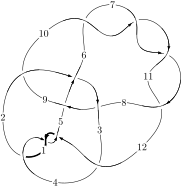
\includegraphics[width=112pt]{../../../GIT/diagram.site/Diagrams/png/1810_12a_1009.png}\\
\ \ \ A knot diagram\footnotemark}&
\allowdisplaybreaks
\textbf{Linearized knot diagam} \\
\cline{2-2}
 &
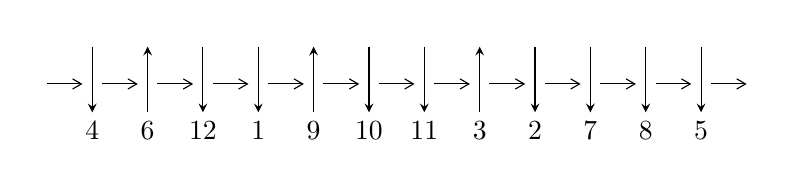
\begin{tikzpicture}[x=20pt, y=17pt]
	% nodes
	\node (C0) at (0, 0) {};
	\node (C1) at (1, 0) {};
	\node (C1U) at (1, +1) {};
	\node (C1D) at (1, -1) {4};

	\node (C2) at (2, 0) {};
	\node (C2U) at (2, +1) {};
	\node (C2D) at (2, -1) {6};

	\node (C3) at (3, 0) {};
	\node (C3U) at (3, +1) {};
	\node (C3D) at (3, -1) {12};

	\node (C4) at (4, 0) {};
	\node (C4U) at (4, +1) {};
	\node (C4D) at (4, -1) {1};

	\node (C5) at (5, 0) {};
	\node (C5U) at (5, +1) {};
	\node (C5D) at (5, -1) {9};

	\node (C6) at (6, 0) {};
	\node (C6U) at (6, +1) {};
	\node (C6D) at (6, -1) {10};

	\node (C7) at (7, 0) {};
	\node (C7U) at (7, +1) {};
	\node (C7D) at (7, -1) {11};

	\node (C8) at (8, 0) {};
	\node (C8U) at (8, +1) {};
	\node (C8D) at (8, -1) {3};

	\node (C9) at (9, 0) {};
	\node (C9U) at (9, +1) {};
	\node (C9D) at (9, -1) {2};

	\node (C10) at (10, 0) {};
	\node (C10U) at (10, +1) {};
	\node (C10D) at (10, -1) {7};

	\node (C11) at (11, 0) {};
	\node (C11U) at (11, +1) {};
	\node (C11D) at (11, -1) {8};

	\node (C12) at (12, 0) {};
	\node (C12U) at (12, +1) {};
	\node (C12D) at (12, -1) {5};
	\node (C13) at (13, 0) {};

	% arrows
	\draw[->,>={angle 60}]
	(C0) edge (C1) (C1) edge (C2) (C2) edge (C3) (C3) edge (C4) (C4) edge (C5) (C5) edge (C6) (C6) edge (C7) (C7) edge (C8) (C8) edge (C9) (C9) edge (C10) (C10) edge (C11) (C11) edge (C12) (C12) edge (C13) ;	\draw[->,>=stealth]
	(C1U) edge (C1D) (C2D) edge (C2U) (C3U) edge (C3D) (C4U) edge (C4D) (C5D) edge (C5U) (C6U) edge (C6D) (C7U) edge (C7D) (C8D) edge (C8U) (C9U) edge (C9D) (C10U) edge (C10D) (C11U) edge (C11D) (C12U) edge (C12D) ;
	\end{tikzpicture} \\
\hhline{~~} \\& 
\textbf{Solving Sequence} \\ \cline{2-2} 
 &
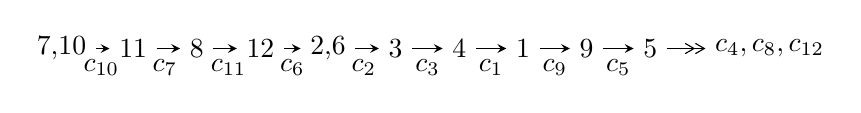
\begin{tikzpicture}[x=23pt, y=7pt]
	% node
	\node (A0) at (-1/8, 0) {7,10};
	\node (A1) at (1, 0) {11};
	\node (A2) at (2, 0) {8};
	\node (A3) at (3, 0) {12};
	\node (A4) at (65/16, 0) {2,6};
	\node (A5) at (41/8, 0) {3};
	\node (A6) at (49/8, 0) {4};
	\node (A7) at (57/8, 0) {1};
	\node (A8) at (65/8, 0) {9};
	\node (A9) at (73/8, 0) {5};
	\node (C1) at (1/2, -1) {$c_{10}$};
	\node (C2) at (3/2, -1) {$c_{7}$};
	\node (C3) at (5/2, -1) {$c_{11}$};
	\node (C4) at (7/2, -1) {$c_{6}$};
	\node (C5) at (37/8, -1) {$c_{2}$};
	\node (C6) at (45/8, -1) {$c_{3}$};
	\node (C7) at (53/8, -1) {$c_{1}$};
	\node (C8) at (61/8, -1) {$c_{9}$};
	\node (C9) at (69/8, -1) {$c_{5}$};
	\node (A10) at (11, 0) {$c_{4},c_{8},c_{12}$};

	% edge
	\draw[->,>=stealth]	
	(A0) edge (A1) (A1) edge (A2) (A2) edge (A3) (A3) edge (A4) (A4) edge (A5) (A5) edge (A6) (A6) edge (A7) (A7) edge (A8) (A8) edge (A9) ;
	\draw[->>,>={angle 60}]	
	(A9) edge (A10);
\end{tikzpicture} \\ 

\end{tabular} \\

\footnotetext{
The image of knot diagram is generated by the software ``\textbf{Draw programme}" developed by Andrew Bartholomew(\url{http://www.layer8.co.uk/maths/draw/index.htm\#Running-draw}), where we modified some parts for our purpose(\url{https://github.com/CATsTAILs/LinksPainter}).
}\phantom \\ \newline 
\centering \textbf{Ideals for irreducible components\footnotemark of $X_{\text{par}}$} 
 
\begin{align*}
I^u_{1}&=\langle 
-2.83377\times10^{70} u^{70}-9.54793\times10^{70} u^{69}+\cdots+1.77999\times10^{69} b+4.28601\times10^{70},\\
\phantom{I^u_{1}}&\phantom{= \langle  }-1.01200\times10^{71} u^{70}-3.39563\times10^{71} u^{69}+\cdots+5.33996\times10^{69} a+1.38029\times10^{71},\\
\phantom{I^u_{1}}&\phantom{= \langle  }u^{71}+4 u^{70}+\cdots-11 u-1\rangle \\
I^u_{2}&=\langle 
b- a,\;a^3- a^2+1,\;u+1\rangle \\
\\
\end{align*}
\raggedright * 2 irreducible components of $\dim_{\mathbb{C}}=0$, with total 74 representations.\\
\footnotetext{All coefficients of polynomials are rational numbers. But the coefficients are sometimes approximated in decimal forms when there is not enough margin.}
\newpage
\renewcommand{\arraystretch}{1}
\centering \section*{I. $I^u_{1}= \langle -2.83\times10^{70} u^{70}-9.55\times10^{70} u^{69}+\cdots+1.78\times10^{69} b+4.29\times10^{70},\;-1.01\times10^{71} u^{70}-3.40\times10^{71} u^{69}+\cdots+5.34\times10^{69} a+1.38\times10^{71},\;u^{71}+4 u^{70}+\cdots-11 u-1 \rangle$}
\flushleft \textbf{(i) Arc colorings}\\
\begin{tabular}{m{7pt} m{180pt} m{7pt} m{180pt} }
\flushright $a_{7}=$&$\begin{pmatrix}0\\u\end{pmatrix}$ \\
\flushright $a_{10}=$&$\begin{pmatrix}1\\0\end{pmatrix}$ \\
\flushright $a_{11}=$&$\begin{pmatrix}1\\u^2\end{pmatrix}$ \\
\flushright $a_{8}=$&$\begin{pmatrix}- u\\- u^3+u\end{pmatrix}$ \\
\flushright $a_{12}=$&$\begin{pmatrix}- u^2+1\\- u^4+2 u^2\end{pmatrix}$ \\
\flushright $a_{2}=$&$\begin{pmatrix}18.9514 u^{70}+63.5891 u^{69}+\cdots-271.927 u-25.8484\\15.9202 u^{70}+53.6404 u^{69}+\cdots-234.194 u-24.0789\end{pmatrix}$ \\
\flushright $a_{6}=$&$\begin{pmatrix}u\\u\end{pmatrix}$ \\
\flushright $a_{3}=$&$\begin{pmatrix}17.2006 u^{70}+58.3127 u^{69}+\cdots-251.019 u-23.6721\\14.1693 u^{70}+48.3641 u^{69}+\cdots-213.286 u-21.9026\end{pmatrix}$ \\
\flushright $a_{4}=$&$\begin{pmatrix}19.8181 u^{70}+66.3472 u^{69}+\cdots-282.283 u-27.5349\\18.5251 u^{70}+62.2805 u^{69}+\cdots-268.012 u-27.5305\end{pmatrix}$ \\
\flushright $a_{1}=$&$\begin{pmatrix}1.01917 u^{70}+3.16140 u^{69}+\cdots-3.40337 u+1.44731\\1.16536 u^{70}+3.78779 u^{69}+\cdots-5.87924 u-0.221025\end{pmatrix}$ \\
\flushright $a_{9}=$&$\begin{pmatrix}5.05082 u^{70}+17.2412 u^{69}+\cdots-52.3212 u-5.84505\\6.62995 u^{70}+22.6456 u^{69}+\cdots-101.441 u-10.8064\end{pmatrix}$ \\
\flushright $a_{5}=$&$\begin{pmatrix}2.46549 u^{70}+7.58181 u^{69}+\cdots-26.3911 u-4.12137\\2.46549 u^{70}+7.58181 u^{69}+\cdots-26.3911 u-3.12137\end{pmatrix}$\\&\end{tabular}
\flushleft \textbf{(ii) Obstruction class $= -1$}\\~\\
\flushleft \textbf{(iii) Cusp Shapes $= -97.9174 u^{70}-336.151 u^{69}+\cdots+1510.09 u+154.499$}\\~\\
\newpage\renewcommand{\arraystretch}{1}
\flushleft \textbf{(iv) u-Polynomials at the component}\newline \\
\begin{tabular}{m{50pt}|m{274pt}}
Crossings & \hspace{64pt}u-Polynomials at each crossing \\
\hline $$\begin{aligned}c_{1},c_{4},c_{12}\end{aligned}$$&$\begin{aligned}
&u^{71}-2 u^{70}+\cdots-8 u-1
\end{aligned}$\\
\hline $$\begin{aligned}c_{2}\end{aligned}$$&$\begin{aligned}
&u^{71}-5 u^{70}+\cdots+12 u-8
\end{aligned}$\\
\hline $$\begin{aligned}c_{3}\end{aligned}$$&$\begin{aligned}
&u^{71}+2 u^{70}+\cdots-14304 u-929
\end{aligned}$\\
\hline $$\begin{aligned}c_{5}\end{aligned}$$&$\begin{aligned}
&u^{71}-4 u^{70}+\cdots+3 u-1
\end{aligned}$\\
\hline $$\begin{aligned}c_{6},c_{7},c_{10}\\c_{11}\end{aligned}$$&$\begin{aligned}
&u^{71}+4 u^{70}+\cdots-11 u-1
\end{aligned}$\\
\hline $$\begin{aligned}c_{8}\end{aligned}$$&$\begin{aligned}
&u^{71}-22 u^{69}+\cdots-460924 u-201793
\end{aligned}$\\
\hline $$\begin{aligned}c_{9}\end{aligned}$$&$\begin{aligned}
&u^{71}-2 u^{70}+\cdots-1978 u-169
\end{aligned}$\\
\hline
\end{tabular}\\~\\
\newpage\renewcommand{\arraystretch}{1}
\flushleft \textbf{(v) Riley Polynomials at the component}\newline \\
\begin{tabular}{m{50pt}|m{274pt}}
Crossings & \hspace{64pt}Riley Polynomials at each crossing \\
\hline $$\begin{aligned}c_{1},c_{4},c_{12}\end{aligned}$$&$\begin{aligned}
&y^{71}+60 y^{70}+\cdots+40 y-1
\end{aligned}$\\
\hline $$\begin{aligned}c_{2}\end{aligned}$$&$\begin{aligned}
&y^{71}+21 y^{70}+\cdots+720 y-64
\end{aligned}$\\
\hline $$\begin{aligned}c_{3}\end{aligned}$$&$\begin{aligned}
&y^{71}-36 y^{70}+\cdots+30160512 y-863041
\end{aligned}$\\
\hline $$\begin{aligned}c_{5}\end{aligned}$$&$\begin{aligned}
&y^{71}+2 y^{70}+\cdots-3 y-1
\end{aligned}$\\
\hline $$\begin{aligned}c_{6},c_{7},c_{10}\\c_{11}\end{aligned}$$&$\begin{aligned}
&y^{71}-86 y^{70}+\cdots-3 y-1
\end{aligned}$\\
\hline $$\begin{aligned}c_{8}\end{aligned}$$&$\begin{aligned}
&y^{71}-44 y^{70}+\cdots-833663350352 y-40720414849
\end{aligned}$\\
\hline $$\begin{aligned}c_{9}\end{aligned}$$&$\begin{aligned}
&y^{71}-96 y^{70}+\cdots+7503396 y-28561
\end{aligned}$\\
\hline
\end{tabular}\\~\\
\newpage\flushleft \textbf{(vi) Complex Volumes and Cusp Shapes}
$$\begin{array}{c|c|c}  
\text{Solutions to }I^u_{1}& \I (\text{vol} + \sqrt{-1}CS) & \text{Cusp shape}\\
 \hline 
\begin{aligned}
u &= \phantom{-}0.916330 + 0.404967 I \\
a &= \phantom{-}1.41839 - 0.68949 I \\
b &= \phantom{-}1.089920 + 0.667509 I\end{aligned}
 & -2.48396 - 4.29702 I & \phantom{-0.000000 } 0 \\ \hline\begin{aligned}
u &= \phantom{-}0.916330 - 0.404967 I \\
a &= \phantom{-}1.41839 + 0.68949 I \\
b &= \phantom{-}1.089920 - 0.667509 I\end{aligned}
 & -2.48396 + 4.29702 I & \phantom{-0.000000 } 0 \\ \hline\begin{aligned}
u &= -0.797905 + 0.667654 I \\
a &= \phantom{-}0.407468 + 0.747440 I \\
b &= \phantom{-}0.939564 + 0.123379 I\end{aligned}
 & -0.64412 + 3.87490 I & \phantom{-0.000000 } 0 \\ \hline\begin{aligned}
u &= -0.797905 - 0.667654 I \\
a &= \phantom{-}0.407468 - 0.747440 I \\
b &= \phantom{-}0.939564 - 0.123379 I\end{aligned}
 & -0.64412 - 3.87490 I & \phantom{-0.000000 } 0 \\ \hline\begin{aligned}
u &= \phantom{-}0.919544 + 0.509968 I \\
a &= -1.38427 + 0.50220 I \\
b &= -1.18719 - 0.81000 I\end{aligned}
 & -4.93660 - 8.62281 I & \phantom{-0.000000 } 0 \\ \hline\begin{aligned}
u &= \phantom{-}0.919544 - 0.509968 I \\
a &= -1.38427 - 0.50220 I \\
b &= -1.18719 + 0.81000 I\end{aligned}
 & -4.93660 + 8.62281 I & \phantom{-0.000000 } 0 \\ \hline\begin{aligned}
u &= \phantom{-}0.899669 + 0.567468 I \\
a &= \phantom{-}1.343630 - 0.396527 I \\
b &= \phantom{-}1.21545 + 0.90921 I\end{aligned}
 & \phantom{-}0.03199 - 12.75630 I & \phantom{-0.000000 } 0 \\ \hline\begin{aligned}
u &= \phantom{-}0.899669 - 0.567468 I \\
a &= \phantom{-}1.343630 + 0.396527 I \\
b &= \phantom{-}1.21545 - 0.90921 I\end{aligned}
 & \phantom{-}0.03199 + 12.75630 I & \phantom{-0.000000 } 0 \\ \hline\begin{aligned}
u &= -0.902665 + 0.602685 I \\
a &= -0.299774 - 0.774692 I \\
b &= -0.802092 - 0.207826 I\end{aligned}
 & -4.42813 + 0.27103 I & \phantom{-0.000000 } 0 \\ \hline\begin{aligned}
u &= -0.902665 - 0.602685 I \\
a &= -0.299774 + 0.774692 I \\
b &= -0.802092 + 0.207826 I\end{aligned}
 & -4.42813 - 0.27103 I & \phantom{-0.000000 } 0\\
 \hline 
 \end{array}$$\newpage$$\begin{array}{c|c|c}  
\text{Solutions to }I^u_{1}& \I (\text{vol} + \sqrt{-1}CS) & \text{Cusp shape}\\
 \hline 
\begin{aligned}
u &= -1.16620\phantom{ +0.000000I} \\
a &= -0.362381\phantom{ +0.000000I} \\
b &= \phantom{-}0.0637371\phantom{ +0.000000I}\end{aligned}
 & -2.18683\phantom{ +0.000000I} & \phantom{-0.000000 } 0 \\ \hline\begin{aligned}
u &= -1.013430 + 0.583657 I \\
a &= \phantom{-}0.183762 + 0.842968 I \\
b &= \phantom{-}0.696701 + 0.328940 I\end{aligned}
 & -0.31480 - 3.35362 I & \phantom{-0.000000 } 0 \\ \hline\begin{aligned}
u &= -1.013430 - 0.583657 I \\
a &= \phantom{-}0.183762 - 0.842968 I \\
b &= \phantom{-}0.696701 - 0.328940 I\end{aligned}
 & -0.31480 + 3.35362 I & \phantom{-0.000000 } 0 \\ \hline\begin{aligned}
u &= \phantom{-}0.811667 + 0.167450 I \\
a &= \phantom{-}1.56180 - 1.25295 I \\
b &= \phantom{-}0.749957 + 0.379899 I\end{aligned}
 & -1.94355 - 3.45136 I & \phantom{-0.000000 } 0 \\ \hline\begin{aligned}
u &= \phantom{-}0.811667 - 0.167450 I \\
a &= \phantom{-}1.56180 + 1.25295 I \\
b &= \phantom{-}0.749957 - 0.379899 I\end{aligned}
 & -1.94355 + 3.45136 I & \phantom{-0.000000 } 0 \\ \hline\begin{aligned}
u &= \phantom{-}0.012443 + 0.826554 I \\
a &= \phantom{-}0.185238 - 0.013310 I \\
b &= -0.906553 + 0.727576 I\end{aligned}
 & \phantom{-}2.73486 + 8.14282 I & \phantom{-0.000000 } 0 \\ \hline\begin{aligned}
u &= \phantom{-}0.012443 - 0.826554 I \\
a &= \phantom{-}0.185238 + 0.013310 I \\
b &= -0.906553 - 0.727576 I\end{aligned}
 & \phantom{-}2.73486 - 8.14282 I & \phantom{-0.000000 } 0 \\ \hline\begin{aligned}
u &= \phantom{-}0.788810 + 0.056736 I \\
a &= -2.20931 - 1.28447 I \\
b &= -0.586607 - 0.039795 I\end{aligned}
 & -3.91288 - 1.17863 I & -20.7772 + 5.1029 I \\ \hline\begin{aligned}
u &= \phantom{-}0.788810 - 0.056736 I \\
a &= -2.20931 + 1.28447 I \\
b &= -0.586607 + 0.039795 I\end{aligned}
 & -3.91288 + 1.17863 I & -20.7772 - 5.1029 I \\ \hline\begin{aligned}
u &= \phantom{-}0.750230 + 0.210776 I \\
a &= \phantom{-}2.28809 + 0.97667 I \\
b &= \phantom{-}0.475905 + 0.328068 I\end{aligned}
 & \phantom{-}1.15173 - 5.50599 I & -6.00000 + 10.13859 I\\
 \hline 
 \end{array}$$\newpage$$\begin{array}{c|c|c}  
\text{Solutions to }I^u_{1}& \I (\text{vol} + \sqrt{-1}CS) & \text{Cusp shape}\\
 \hline 
\begin{aligned}
u &= \phantom{-}0.750230 - 0.210776 I \\
a &= \phantom{-}2.28809 - 0.97667 I \\
b &= \phantom{-}0.475905 - 0.328068 I\end{aligned}
 & \phantom{-}1.15173 + 5.50599 I & -6.00000 - 10.13859 I \\ \hline\begin{aligned}
u &= -0.057589 + 0.774983 I \\
a &= -0.130444 + 0.204956 I \\
b &= \phantom{-}0.917161 - 0.614056 I\end{aligned}
 & -1.95781 + 4.36004 I & -9.73775 - 6.33857 I \\ \hline\begin{aligned}
u &= -0.057589 - 0.774983 I \\
a &= -0.130444 - 0.204956 I \\
b &= \phantom{-}0.917161 + 0.614056 I\end{aligned}
 & -1.95781 - 4.36004 I & -9.73775 + 6.33857 I \\ \hline\begin{aligned}
u &= \phantom{-}0.642028 + 0.410757 I \\
a &= -0.750353 + 0.843964 I \\
b &= -0.684830 - 0.915401 I\end{aligned}
 & \phantom{-}5.36047 - 4.61297 I & -2.63206 + 7.81095 I \\ \hline\begin{aligned}
u &= \phantom{-}0.642028 - 0.410757 I \\
a &= -0.750353 - 0.843964 I \\
b &= -0.684830 + 0.915401 I\end{aligned}
 & \phantom{-}5.36047 + 4.61297 I & -2.63206 - 7.81095 I \\ \hline\begin{aligned}
u &= -0.221305 + 0.702040 I \\
a &= -0.093157 - 0.497861 I \\
b &= -0.965469 + 0.417790 I\end{aligned}
 & \phantom{-}0.956547 + 0.819716 I & -7.05042 - 3.17652 I \\ \hline\begin{aligned}
u &= -0.221305 - 0.702040 I \\
a &= -0.093157 + 0.497861 I \\
b &= -0.965469 - 0.417790 I\end{aligned}
 & \phantom{-}0.956547 - 0.819716 I & -7.05042 + 3.17652 I \\ \hline\begin{aligned}
u &= -1.253580 + 0.245545 I \\
a &= \phantom{-}0.451351 - 0.533518 I \\
b &= -0.095832 - 0.256473 I\end{aligned}
 & \phantom{-}1.87673 + 1.66795 I & \phantom{-0.000000 } 0 \\ \hline\begin{aligned}
u &= -1.253580 - 0.245545 I \\
a &= \phantom{-}0.451351 + 0.533518 I \\
b &= -0.095832 + 0.256473 I\end{aligned}
 & \phantom{-}1.87673 - 1.66795 I & \phantom{-0.000000 } 0 \\ \hline\begin{aligned}
u &= -0.689252 + 0.066561 I \\
a &= \phantom{-}3.77196 - 0.35800 I \\
b &= \phantom{-}3.28529 - 0.34701 I\end{aligned}
 & \phantom{-}1.80845 + 2.97035 I & \phantom{-}27.2900 + 10.8535 I\\
 \hline 
 \end{array}$$\newpage$$\begin{array}{c|c|c}  
\text{Solutions to }I^u_{1}& \I (\text{vol} + \sqrt{-1}CS) & \text{Cusp shape}\\
 \hline 
\begin{aligned}
u &= -0.689252 - 0.066561 I \\
a &= \phantom{-}3.77196 + 0.35800 I \\
b &= \phantom{-}3.28529 + 0.34701 I\end{aligned}
 & \phantom{-}1.80845 - 2.97035 I & \phantom{-}27.2900 - 10.8535 I \\ \hline\begin{aligned}
u &= -0.674572\phantom{ +0.000000I} \\
a &= -3.82901\phantom{ +0.000000I} \\
b &= -3.39142\phantom{ +0.000000I}\end{aligned}
 & -2.27556\phantom{ +0.000000I} & \phantom{-}45.0080\phantom{ +0.000000I} \\ \hline\begin{aligned}
u &= -0.649970 + 0.157969 I \\
a &= \phantom{-}0.715941 + 0.100560 I \\
b &= \phantom{-}0.728948 - 0.515381 I\end{aligned}
 & -1.239550 + 0.397962 I & -8.72729 - 0.25235 I \\ \hline\begin{aligned}
u &= -0.649970 - 0.157969 I \\
a &= \phantom{-}0.715941 - 0.100560 I \\
b &= \phantom{-}0.728948 + 0.515381 I\end{aligned}
 & -1.239550 - 0.397962 I & -8.72729 + 0.25235 I \\ \hline\begin{aligned}
u &= \phantom{-}0.248104 + 0.573900 I \\
a &= -1.127820 + 0.073338 I \\
b &= \phantom{-}0.440596 - 0.654495 I\end{aligned}
 & \phantom{-}6.54466 + 1.22183 I & \phantom{-}0.937262 - 0.719785 I \\ \hline\begin{aligned}
u &= \phantom{-}0.248104 - 0.573900 I \\
a &= -1.127820 - 0.073338 I \\
b &= \phantom{-}0.440596 + 0.654495 I\end{aligned}
 & \phantom{-}6.54466 - 1.22183 I & \phantom{-}0.937262 + 0.719785 I \\ \hline\begin{aligned}
u &= -0.418442 + 0.184487 I \\
a &= -2.67657 + 0.89298 I \\
b &= -1.54879 + 0.72191 I\end{aligned}
 & \phantom{-}2.23688 - 2.23181 I & -2.34161 + 7.40187 I \\ \hline\begin{aligned}
u &= -0.418442 - 0.184487 I \\
a &= -2.67657 - 0.89298 I \\
b &= -1.54879 - 0.72191 I\end{aligned}
 & \phantom{-}2.23688 + 2.23181 I & -2.34161 - 7.40187 I \\ \hline\begin{aligned}
u &= \phantom{-}1.54364 + 0.03606 I \\
a &= \phantom{-}2.07634 + 0.16337 I \\
b &= \phantom{-}1.72830 + 0.61768 I\end{aligned}
 & -4.29068 - 2.11335 I & \phantom{-0.000000 } 0 \\ \hline\begin{aligned}
u &= \phantom{-}1.54364 - 0.03606 I \\
a &= \phantom{-}2.07634 - 0.16337 I \\
b &= \phantom{-}1.72830 - 0.61768 I\end{aligned}
 & -4.29068 + 2.11335 I & \phantom{-0.000000 } 0\\
 \hline 
 \end{array}$$\newpage$$\begin{array}{c|c|c}  
\text{Solutions to }I^u_{1}& \I (\text{vol} + \sqrt{-1}CS) & \text{Cusp shape}\\
 \hline 
\begin{aligned}
u &= -0.027766 + 0.439550 I \\
a &= \phantom{-}0.616350 - 1.062520 I \\
b &= -0.655258 + 0.345763 I\end{aligned}
 & \phantom{-}0.73320 + 1.40973 I & -1.20605 - 3.84392 I \\ \hline\begin{aligned}
u &= -0.027766 - 0.439550 I \\
a &= \phantom{-}0.616350 + 1.062520 I \\
b &= -0.655258 - 0.345763 I\end{aligned}
 & \phantom{-}0.73320 - 1.40973 I & -1.20605 + 3.84392 I \\ \hline\begin{aligned}
u &= -1.60578 + 0.08607 I \\
a &= \phantom{-}1.287790 - 0.085996 I \\
b &= \phantom{-}0.851120 - 1.100430 I\end{aligned}
 & -2.34616 + 6.29316 I & \phantom{-0.000000 } 0 \\ \hline\begin{aligned}
u &= -1.60578 - 0.08607 I \\
a &= \phantom{-}1.287790 + 0.085996 I \\
b &= \phantom{-}0.851120 + 1.100430 I\end{aligned}
 & -2.34616 - 6.29316 I & \phantom{-0.000000 } 0 \\ \hline\begin{aligned}
u &= \phantom{-}1.62936 + 0.03391 I \\
a &= -1.093500 - 0.875100 I \\
b &= -0.96393 - 1.30038 I\end{aligned}
 & -9.26887 - 1.05823 I & \phantom{-0.000000 } 0 \\ \hline\begin{aligned}
u &= \phantom{-}1.62936 - 0.03391 I \\
a &= -1.093500 + 0.875100 I \\
b &= -0.96393 + 1.30038 I\end{aligned}
 & -9.26887 + 1.05823 I & \phantom{-0.000000 } 0 \\ \hline\begin{aligned}
u &= \phantom{-}1.63403\phantom{ +0.000000I} \\
a &= \phantom{-}3.86249\phantom{ +0.000000I} \\
b &= \phantom{-}3.49963\phantom{ +0.000000I}\end{aligned}
 & -10.4426\phantom{ +0.000000I} & \phantom{-0.000000 } 0 \\ \hline\begin{aligned}
u &= \phantom{-}1.63409 + 0.02399 I \\
a &= -3.55343 + 0.22314 I \\
b &= -3.14434 + 0.32055 I\end{aligned}
 & -6.38831 - 3.34830 I & \phantom{-0.000000 } 0 \\ \hline\begin{aligned}
u &= \phantom{-}1.63409 - 0.02399 I \\
a &= -3.55343 - 0.22314 I \\
b &= -3.14434 - 0.32055 I\end{aligned}
 & -6.38831 + 3.34830 I & \phantom{-0.000000 } 0 \\ \hline\begin{aligned}
u &= -1.64131 + 0.04793 I \\
a &= -1.75205 + 0.63284 I \\
b &= -0.658185 - 0.009831 I\end{aligned}
 & -7.20909 + 6.42648 I & \phantom{-0.000000 } 0\\
 \hline 
 \end{array}$$\newpage$$\begin{array}{c|c|c}  
\text{Solutions to }I^u_{1}& \I (\text{vol} + \sqrt{-1}CS) & \text{Cusp shape}\\
 \hline 
\begin{aligned}
u &= -1.64131 - 0.04793 I \\
a &= -1.75205 - 0.63284 I \\
b &= -0.658185 + 0.009831 I\end{aligned}
 & -7.20909 - 6.42648 I & \phantom{-0.000000 } 0 \\ \hline\begin{aligned}
u &= -1.65355 + 0.01136 I \\
a &= \phantom{-}1.75280 - 0.69764 I \\
b &= \phantom{-}0.698957 + 0.215320 I\end{aligned}
 & -12.50500 + 1.41291 I & \phantom{-0.000000 } 0 \\ \hline\begin{aligned}
u &= -1.65355 - 0.01136 I \\
a &= \phantom{-}1.75280 + 0.69764 I \\
b &= \phantom{-}0.698957 - 0.215320 I\end{aligned}
 & -12.50500 - 1.41291 I & \phantom{-0.000000 } 0 \\ \hline\begin{aligned}
u &= -1.65390 + 0.03334 I \\
a &= -1.55282 - 0.51867 I \\
b &= -0.800340 + 0.545581 I\end{aligned}
 & -10.56950 + 4.14320 I & \phantom{-0.000000 } 0 \\ \hline\begin{aligned}
u &= -1.65390 - 0.03334 I \\
a &= -1.55282 + 0.51867 I \\
b &= -0.800340 - 0.545581 I\end{aligned}
 & -10.56950 - 4.14320 I & \phantom{-0.000000 } 0 \\ \hline\begin{aligned}
u &= -1.67951 + 0.11538 I \\
a &= -1.84477 - 0.04028 I \\
b &= -1.28310 + 0.83407 I\end{aligned}
 & -11.49190 + 6.36006 I & \phantom{-0.000000 } 0 \\ \hline\begin{aligned}
u &= -1.67951 - 0.11538 I \\
a &= -1.84477 + 0.04028 I \\
b &= -1.28310 - 0.83407 I\end{aligned}
 & -11.49190 - 6.36006 I & \phantom{-0.000000 } 0 \\ \hline\begin{aligned}
u &= \phantom{-}1.67267 + 0.19634 I \\
a &= -1.242390 + 0.481250 I \\
b &= -1.087260 - 0.168561 I\end{aligned}
 & -9.10774 - 7.22720 I & \phantom{-0.000000 } 0 \\ \hline\begin{aligned}
u &= \phantom{-}1.67267 - 0.19634 I \\
a &= -1.242390 - 0.481250 I \\
b &= -1.087260 + 0.168561 I\end{aligned}
 & -9.10774 + 7.22720 I & \phantom{-0.000000 } 0 \\ \hline\begin{aligned}
u &= -1.67935 + 0.16443 I \\
a &= -2.00330 + 0.17615 I \\
b &= -1.48667 + 0.99930 I\end{aligned}
 & -8.8172 + 15.6243 I & \phantom{-0.000000 } 0\\
 \hline 
 \end{array}$$\newpage$$\begin{array}{c|c|c}  
\text{Solutions to }I^u_{1}& \I (\text{vol} + \sqrt{-1}CS) & \text{Cusp shape}\\
 \hline 
\begin{aligned}
u &= -1.67935 - 0.16443 I \\
a &= -2.00330 - 0.17615 I \\
b &= -1.48667 - 0.99930 I\end{aligned}
 & -8.8172 - 15.6243 I & \phantom{-0.000000 } 0 \\ \hline\begin{aligned}
u &= -1.68414 + 0.14421 I \\
a &= \phantom{-}1.95556 - 0.07671 I \\
b &= \phantom{-}1.41912 - 0.91577 I\end{aligned}
 & -13.9245 + 11.1963 I & \phantom{-0.000000 } 0 \\ \hline\begin{aligned}
u &= -1.68414 - 0.14421 I \\
a &= \phantom{-}1.95556 + 0.07671 I \\
b &= \phantom{-}1.41912 + 0.91577 I\end{aligned}
 & -13.9245 - 11.1963 I & \phantom{-0.000000 } 0 \\ \hline\begin{aligned}
u &= \phantom{-}1.69608 + 0.16003 I \\
a &= \phantom{-}1.070460 - 0.423461 I \\
b &= \phantom{-}0.938968 + 0.203592 I\end{aligned}
 & -13.44530 - 3.25448 I & \phantom{-0.000000 } 0 \\ \hline\begin{aligned}
u &= \phantom{-}1.69608 - 0.16003 I \\
a &= \phantom{-}1.070460 + 0.423461 I \\
b &= \phantom{-}0.938968 - 0.203592 I\end{aligned}
 & -13.44530 + 3.25448 I & \phantom{-0.000000 } 0 \\ \hline\begin{aligned}
u &= -0.008362 + 0.294687 I \\
a &= -2.44024 - 0.48075 I \\
b &= -0.419854 + 1.049640 I\end{aligned}
 & \phantom{-}3.27067 + 3.66399 I & -0.860825 - 0.895430 I \\ \hline\begin{aligned}
u &= -0.008362 - 0.294687 I \\
a &= -2.44024 + 0.48075 I \\
b &= -0.419854 - 1.049640 I\end{aligned}
 & \phantom{-}3.27067 - 3.66399 I & -0.860825 + 0.895430 I \\ \hline\begin{aligned}
u &= \phantom{-}1.72348 + 0.11551 I \\
a &= -0.803597 + 0.371179 I \\
b &= -0.707949 - 0.235462 I\end{aligned}
 & -10.04190 + 0.66192 I & \phantom{-0.000000 } 0 \\ \hline\begin{aligned}
u &= \phantom{-}1.72348 - 0.11551 I \\
a &= -0.803597 - 0.371179 I \\
b &= -0.707949 + 0.235462 I\end{aligned}
 & -10.04190 - 0.66192 I & \phantom{-0.000000 } 0 \\ \hline\begin{aligned}
u &= -0.146978 + 0.147957 I \\
a &= \phantom{-}3.53532 - 0.76333 I \\
b &= \phantom{-}0.722322 - 0.678600 I\end{aligned}
 & -1.35611 + 0.52258 I & -7.48776 + 0.18415 I\\
 \hline 
 \end{array}$$\newpage$$\begin{array}{c|c|c}  
\text{Solutions to }I^u_{1}& \I (\text{vol} + \sqrt{-1}CS) & \text{Cusp shape}\\
 \hline 
\begin{aligned}
u &= -0.146978 - 0.147957 I \\
a &= \phantom{-}3.53532 + 0.76333 I \\
b &= \phantom{-}0.722322 + 0.678600 I\end{aligned}
 & -1.35611 - 0.52258 I & -7.48776 - 0.18415 I\\
 \hline 
 \end{array}$$\newpage\newpage\renewcommand{\arraystretch}{1}
\centering \section*{II. $I^u_{2}= \langle b- a,\;a^3- a^2+1,\;u+1 \rangle$}
\flushleft \textbf{(i) Arc colorings}\\
\begin{tabular}{m{7pt} m{180pt} m{7pt} m{180pt} }
\flushright $a_{7}=$&$\begin{pmatrix}0\\-1\end{pmatrix}$ \\
\flushright $a_{10}=$&$\begin{pmatrix}1\\0\end{pmatrix}$ \\
\flushright $a_{11}=$&$\begin{pmatrix}1\\1\end{pmatrix}$ \\
\flushright $a_{8}=$&$\begin{pmatrix}1\\0\end{pmatrix}$ \\
\flushright $a_{12}=$&$\begin{pmatrix}0\\1\end{pmatrix}$ \\
\flushright $a_{2}=$&$\begin{pmatrix}a\\a\end{pmatrix}$ \\
\flushright $a_{6}=$&$\begin{pmatrix}-1\\-1\end{pmatrix}$ \\
\flushright $a_{3}=$&$\begin{pmatrix}a\\a\end{pmatrix}$ \\
\flushright $a_{4}=$&$\begin{pmatrix}a\\2 a\end{pmatrix}$ \\
\flushright $a_{1}=$&$\begin{pmatrix}- a^2+a+1\\-2 a^2+a+2\end{pmatrix}$ \\
\flushright $a_{9}=$&$\begin{pmatrix}- a^2+1\\- a^2\end{pmatrix}$ \\
\flushright $a_{5}=$&$\begin{pmatrix}- a^2\\- a^2-1\end{pmatrix}$\\&\end{tabular}
\flushleft \textbf{(ii) Obstruction class $= 1$}\\~\\
\flushleft \textbf{(iii) Cusp Shapes $= - a^2+5 a-11$}\\~\\
\newpage\renewcommand{\arraystretch}{1}
\flushleft \textbf{(iv) u-Polynomials at the component}\newline \\
\begin{tabular}{m{50pt}|m{274pt}}
Crossings & \hspace{64pt}u-Polynomials at each crossing \\
\hline $$\begin{aligned}c_{1},c_{12}\end{aligned}$$&$\begin{aligned}
&u^3- u^2+2 u-1
\end{aligned}$\\
\hline $$\begin{aligned}c_{2}\end{aligned}$$&$\begin{aligned}
&u^3
\end{aligned}$\\
\hline $$\begin{aligned}c_{3},c_{8},c_{9}\end{aligned}$$&$\begin{aligned}
&u^3- u^2+1
\end{aligned}$\\
\hline $$\begin{aligned}c_{4}\end{aligned}$$&$\begin{aligned}
&u^3+u^2+2 u+1
\end{aligned}$\\
\hline $$\begin{aligned}c_{5},c_{6},c_{7}\end{aligned}$$&$\begin{aligned}
&(u-1)^3
\end{aligned}$\\
\hline $$\begin{aligned}c_{10},c_{11}\end{aligned}$$&$\begin{aligned}
&(u+1)^3
\end{aligned}$\\
\hline
\end{tabular}\\~\\
\newpage\renewcommand{\arraystretch}{1}
\flushleft \textbf{(v) Riley Polynomials at the component}\newline \\
\begin{tabular}{m{50pt}|m{274pt}}
Crossings & \hspace{64pt}Riley Polynomials at each crossing \\
\hline $$\begin{aligned}c_{1},c_{4},c_{12}\end{aligned}$$&$\begin{aligned}
&y^3+3 y^2+2 y-1
\end{aligned}$\\
\hline $$\begin{aligned}c_{2}\end{aligned}$$&$\begin{aligned}
&y^3
\end{aligned}$\\
\hline $$\begin{aligned}c_{3},c_{8},c_{9}\end{aligned}$$&$\begin{aligned}
&y^3- y^2+2 y-1
\end{aligned}$\\
\hline $$\begin{aligned}c_{5},c_{6},c_{7}\\c_{10},c_{11}\end{aligned}$$&$\begin{aligned}
&(y-1)^3
\end{aligned}$\\
\hline
\end{tabular}\\~\\
\newpage\flushleft \textbf{(vi) Complex Volumes and Cusp Shapes}
$$\begin{array}{c|c|c}  
\text{Solutions to }I^u_{2}& \I (\text{vol} + \sqrt{-1}CS) & \text{Cusp shape}\\
 \hline 
\begin{aligned}
u &= -1.00000\phantom{ +0.000000I} \\
a &= \phantom{-}0.877439 + 0.744862 I \\
b &= \phantom{-}0.877439 + 0.744862 I\end{aligned}
 & \phantom{-}1.37919 - 2.82812 I & -6.82789 + 2.41717 I \\ \hline\begin{aligned}
u &= -1.00000\phantom{ +0.000000I} \\
a &= \phantom{-}0.877439 - 0.744862 I \\
b &= \phantom{-}0.877439 - 0.744862 I\end{aligned}
 & \phantom{-}1.37919 + 2.82812 I & -6.82789 - 2.41717 I \\ \hline\begin{aligned}
u &= -1.00000\phantom{ +0.000000I} \\
a &= -0.754878\phantom{ +0.000000I} \\
b &= -0.754878\phantom{ +0.000000I}\end{aligned}
 & -2.75839\phantom{ +0.000000I} & -15.3440\phantom{ +0.000000I}\\
 \hline 
 \end{array}$$\newpage
\newpage\renewcommand{\arraystretch}{1}
\centering \section*{ III. u-Polynomials}
\begin{tabular}{m{50pt}|m{274pt}}
Crossings & \hspace{64pt}u-Polynomials at each crossing \\
\hline $$\begin{aligned}c_{1},c_{12}\end{aligned}$$&$\begin{aligned}
&(u^3- u^2+2 u-1)(u^{71}-2 u^{70}+\cdots-8 u-1)
\end{aligned}$\\
\hline $$\begin{aligned}c_{2}\end{aligned}$$&$\begin{aligned}
&u^3(u^{71}-5 u^{70}+\cdots+12 u-8)
\end{aligned}$\\
\hline $$\begin{aligned}c_{3}\end{aligned}$$&$\begin{aligned}
&(u^3- u^2+1)(u^{71}+2 u^{70}+\cdots-14304 u-929)
\end{aligned}$\\
\hline $$\begin{aligned}c_{4}\end{aligned}$$&$\begin{aligned}
&(u^3+u^2+2 u+1)(u^{71}-2 u^{70}+\cdots-8 u-1)
\end{aligned}$\\
\hline $$\begin{aligned}c_{5}\end{aligned}$$&$\begin{aligned}
&((u-1)^3)(u^{71}-4 u^{70}+\cdots+3 u-1)
\end{aligned}$\\
\hline $$\begin{aligned}c_{6},c_{7}\end{aligned}$$&$\begin{aligned}
&((u-1)^3)(u^{71}+4 u^{70}+\cdots-11 u-1)
\end{aligned}$\\
\hline $$\begin{aligned}c_{8}\end{aligned}$$&$\begin{aligned}
&(u^3- u^2+1)(u^{71}-22 u^{69}+\cdots-460924 u-201793)
\end{aligned}$\\
\hline $$\begin{aligned}c_{9}\end{aligned}$$&$\begin{aligned}
&(u^3- u^2+1)(u^{71}-2 u^{70}+\cdots-1978 u-169)
\end{aligned}$\\
\hline $$\begin{aligned}c_{10},c_{11}\end{aligned}$$&$\begin{aligned}
&((u+1)^3)(u^{71}+4 u^{70}+\cdots-11 u-1)
\end{aligned}$\\
\hline
\end{tabular}\newpage\renewcommand{\arraystretch}{1}
\centering \section*{ IV. Riley Polynomials}
\begin{tabular}{m{50pt}|m{274pt}}
Crossings & \hspace{64pt}Riley Polynomials at each crossing \\
\hline $$\begin{aligned}c_{1},c_{4},c_{12}\end{aligned}$$&$\begin{aligned}
&(y^3+3 y^2+2 y-1)(y^{71}+60 y^{70}+\cdots+40 y-1)
\end{aligned}$\\
\hline $$\begin{aligned}c_{2}\end{aligned}$$&$\begin{aligned}
&y^3(y^{71}+21 y^{70}+\cdots+720 y-64)
\end{aligned}$\\
\hline $$\begin{aligned}c_{3}\end{aligned}$$&$\begin{aligned}
&(y^3- y^2+2 y-1)(y^{71}-36 y^{70}+\cdots+3.01605\times10^{7} y-863041)
\end{aligned}$\\
\hline $$\begin{aligned}c_{5}\end{aligned}$$&$\begin{aligned}
&((y-1)^3)(y^{71}+2 y^{70}+\cdots-3 y-1)
\end{aligned}$\\
\hline $$\begin{aligned}c_{6},c_{7},c_{10}\\c_{11}\end{aligned}$$&$\begin{aligned}
&((y-1)^3)(y^{71}-86 y^{70}+\cdots-3 y-1)
\end{aligned}$\\
\hline $$\begin{aligned}c_{8}\end{aligned}$$&$\begin{aligned}
&(y^3- y^2+2 y-1)\\
&\cdot(y^{71}-44 y^{70}+\cdots-833663350352 y-40720414849)
\end{aligned}$\\
\hline $$\begin{aligned}c_{9}\end{aligned}$$&$\begin{aligned}
&(y^3- y^2+2 y-1)(y^{71}-96 y^{70}+\cdots+7503396 y-28561)
\end{aligned}$\\
\hline
\end{tabular}
\vskip 2pc
\end{document}